\documentclass[]{spie}  
\usepackage[]{graphicx}
\usepackage{hyperref}
\newcommand{\ror}{\emph{Ruby on Rails}}

\title{Chilean Virtual Observatory services implementation for the ALMA public data} 

\author{Jonathan Antognini\supit{a} and Mauricio Solar\supit{a}, Jorge Ibsen\supit{b}, Mauricio Araya \supit{a}, 
Lars Nyman \supit{b}, Diego Mardones\supit{c}, Camilo Valenzuela\supit{a}, Patricio Ramirez\supit{a}, 
Christopher Fernandez\supit{a}, Mario Garces\supit{a}
\skiplinehalf
\supit{a}Universidad Tecnica Federico Santa Maria, Av Esapana 1680, Valparaiso, Chile; \\
\supit{b}Atacama Large Milimeter/submilimeter Array, Alonso de Cordova 3107, Santiago, Chile \\
\supit{c}Universidad de Chile, Av. Beauchef 850, Santiago, Chile \\
}

\authorinfo{Further author information: (Send correspondence to Jonathan Antognini)\\Jonathan Antognini:
E-mail: jantogni@csrg.cl, Telephone: +56 9 6308 3396}

\begin{document} 
\maketitle 

%%%%%%%%%%%%%%%%%%%%%%%%%%%%%%%%%%%%%%%%%%%%%%%%%%%%%%%%%%%%% 
\begin{abstract}
The success of an observatory is usually measured by its impact in the
scientific community, so a common objective is to provide transparent ways to
access the generated data. The Chilean Virtual Observatory (ChiVO), started
working in the implementation of a prototype, in collaboration with ALMA,
considering the current needs of the Chilean astronomical community, in
addition to the protocols and standards of IVOA, and the comparison of
different existing data access toolkit services. Based on this efforts, a VO
prototype was designed and implemented for the ALMA large scale of data.
\end{abstract}

\keywords{ChiVO, Virtual Observatory, IVOA, ALMA, Flask, RoR, DaCHS}

%%%%%%%%%%%%%%%%%%%%%%%%%%%%%%%%%%%%%%%%%%%%%%%%%%%%%%%%%%%%%
\section{INTRODUCTION}
\label{sec:intro}  % \label{} allows reference to this section

\subsection{Big Data in Astronomy}
\label{sec:bdastronomy}
In recent years, the flood of data problem is visible in both, science and
business environments, becoming more relevant the proper use and management of
what has been called \emph{Big Data}. This concept encompasses the management research
of large amounts of information, and these are not easy to process with the
traditional tools and procedures.  When the data volume reaches TeraBytes to
ZetaBytas ranges, algorithms and procedures should be adapted for its use in
new high-performance computing platforms, with Cloud tools, in a distributed
manner, and on-line.  Additionally, we are not only dealing with large
stationary volumes of data, but also with the frequency in its generation; this
creates new challenges in developing solutions, as are the storage, variability
in the format, and response time.  

Big Data is not a technology in itself, but rather a work approach to obtain
value and benefits of these large volumes of data generated nowadays.   These
are some of the features to consider:
\begin{itemize}
\item How to grasp, manage and make use of them
\item How to ensure, check authenticity and reliability
\item How to share and obtain improvements and benefits
\item How to communicate, simplifying the decision-making and subsequent analysis.
\end{itemize}

One of the domains where the Big Data problem is approaching its turning point
is astronomy.  Its state of the art facilities in operations, such as the
Atacama Large Millimeter/submillimeter (ALMA), and those under construction, as
the Large Synoptic Survey Telescope (LSST), and the Square Kilometer Array
(SKA), produce and will produce large-scale data.  The plan for the year 2020
is to have more than 60 PetaBytes of accessible information for the
astronomical community.

\subsection{Observatories in Chile}
\label{sec:obsinchile}
The privileged atmospheric conditions make Chile one of the most favorable
places to the astronomical scientific research.  There are more than a dozen
wide sweeping astronomical facilities throughout Chile \cite{roadmap}; for example, the
already mentioned ``Atacama Large Millimeter/submillimeter Array'' (ALMA), the
``Very Large Telescope'' (VLT), and in the coming years, the ``European Extremely
Large Telescope'' (E-ELT).  With this last telescope, the expectation is that
Chile will have the 60\% of the global astronomical observational power.

One of the conditions established as country is that $10\%$ of the viewing time
should belong to the Chilean astronomical community; thus, it is justified the
need to develop here an astronomic-informatics platform, for an intelligent
management, and analysis.  The need of a system with these characteristics is
not something new: since $2002$ it has been raised the need to create a Virtual
Observatory (VO), at a national level, as a solution to public access, and
advanced manipulation of the large-scale astronomic data.

The VO paradigm is an international initiative that enables the astronomical
data access, under the responsibility of specialized centres for its storage
and processing, at which both astronomers and regular people may accede.  With
the standardization of methods and information is possible to study the
astronomic registries without requesting new observations, reducing the physical
requirements of instruments and locations, and minimizing data duplication.

\subsection{ALMA data cubes}
\label{sec:almadatacubes}

ALMA is a radio astronomic interferometric observatory, which in simple words
corresponds to the observations of millimeter and submillimeter signals, using
two or more radio antennas.  When combining these signals to analyze them, it is
possible to obtain detailed information of the source of emission (be it
galactic or extra-galactic) with unprecedented resolutions.  In its maximum
operation, it will be possible to combine 66 antennas located in Chajnantor,
Chile, up to $5000$ meters height, which can operate in a wide range of
frequencies, from 84 GHz to 950 GHz (ALMA Band 3 - ALMA Band 10).

From the standpoint of data production, this process generates three-dimmension
cubes given by two position shafts in the celestial vault, and one shaft of
frequency spectrum (see Figure~\ref{fig:cube}).  The uniqueness of these data cubes is their
size, since the spatial and spectral high resolution that this observatory
provides generates large-scale data cubes (from GB and TB).

\begin{figure}
   \begin{center}
   \begin{tabular}{c}
   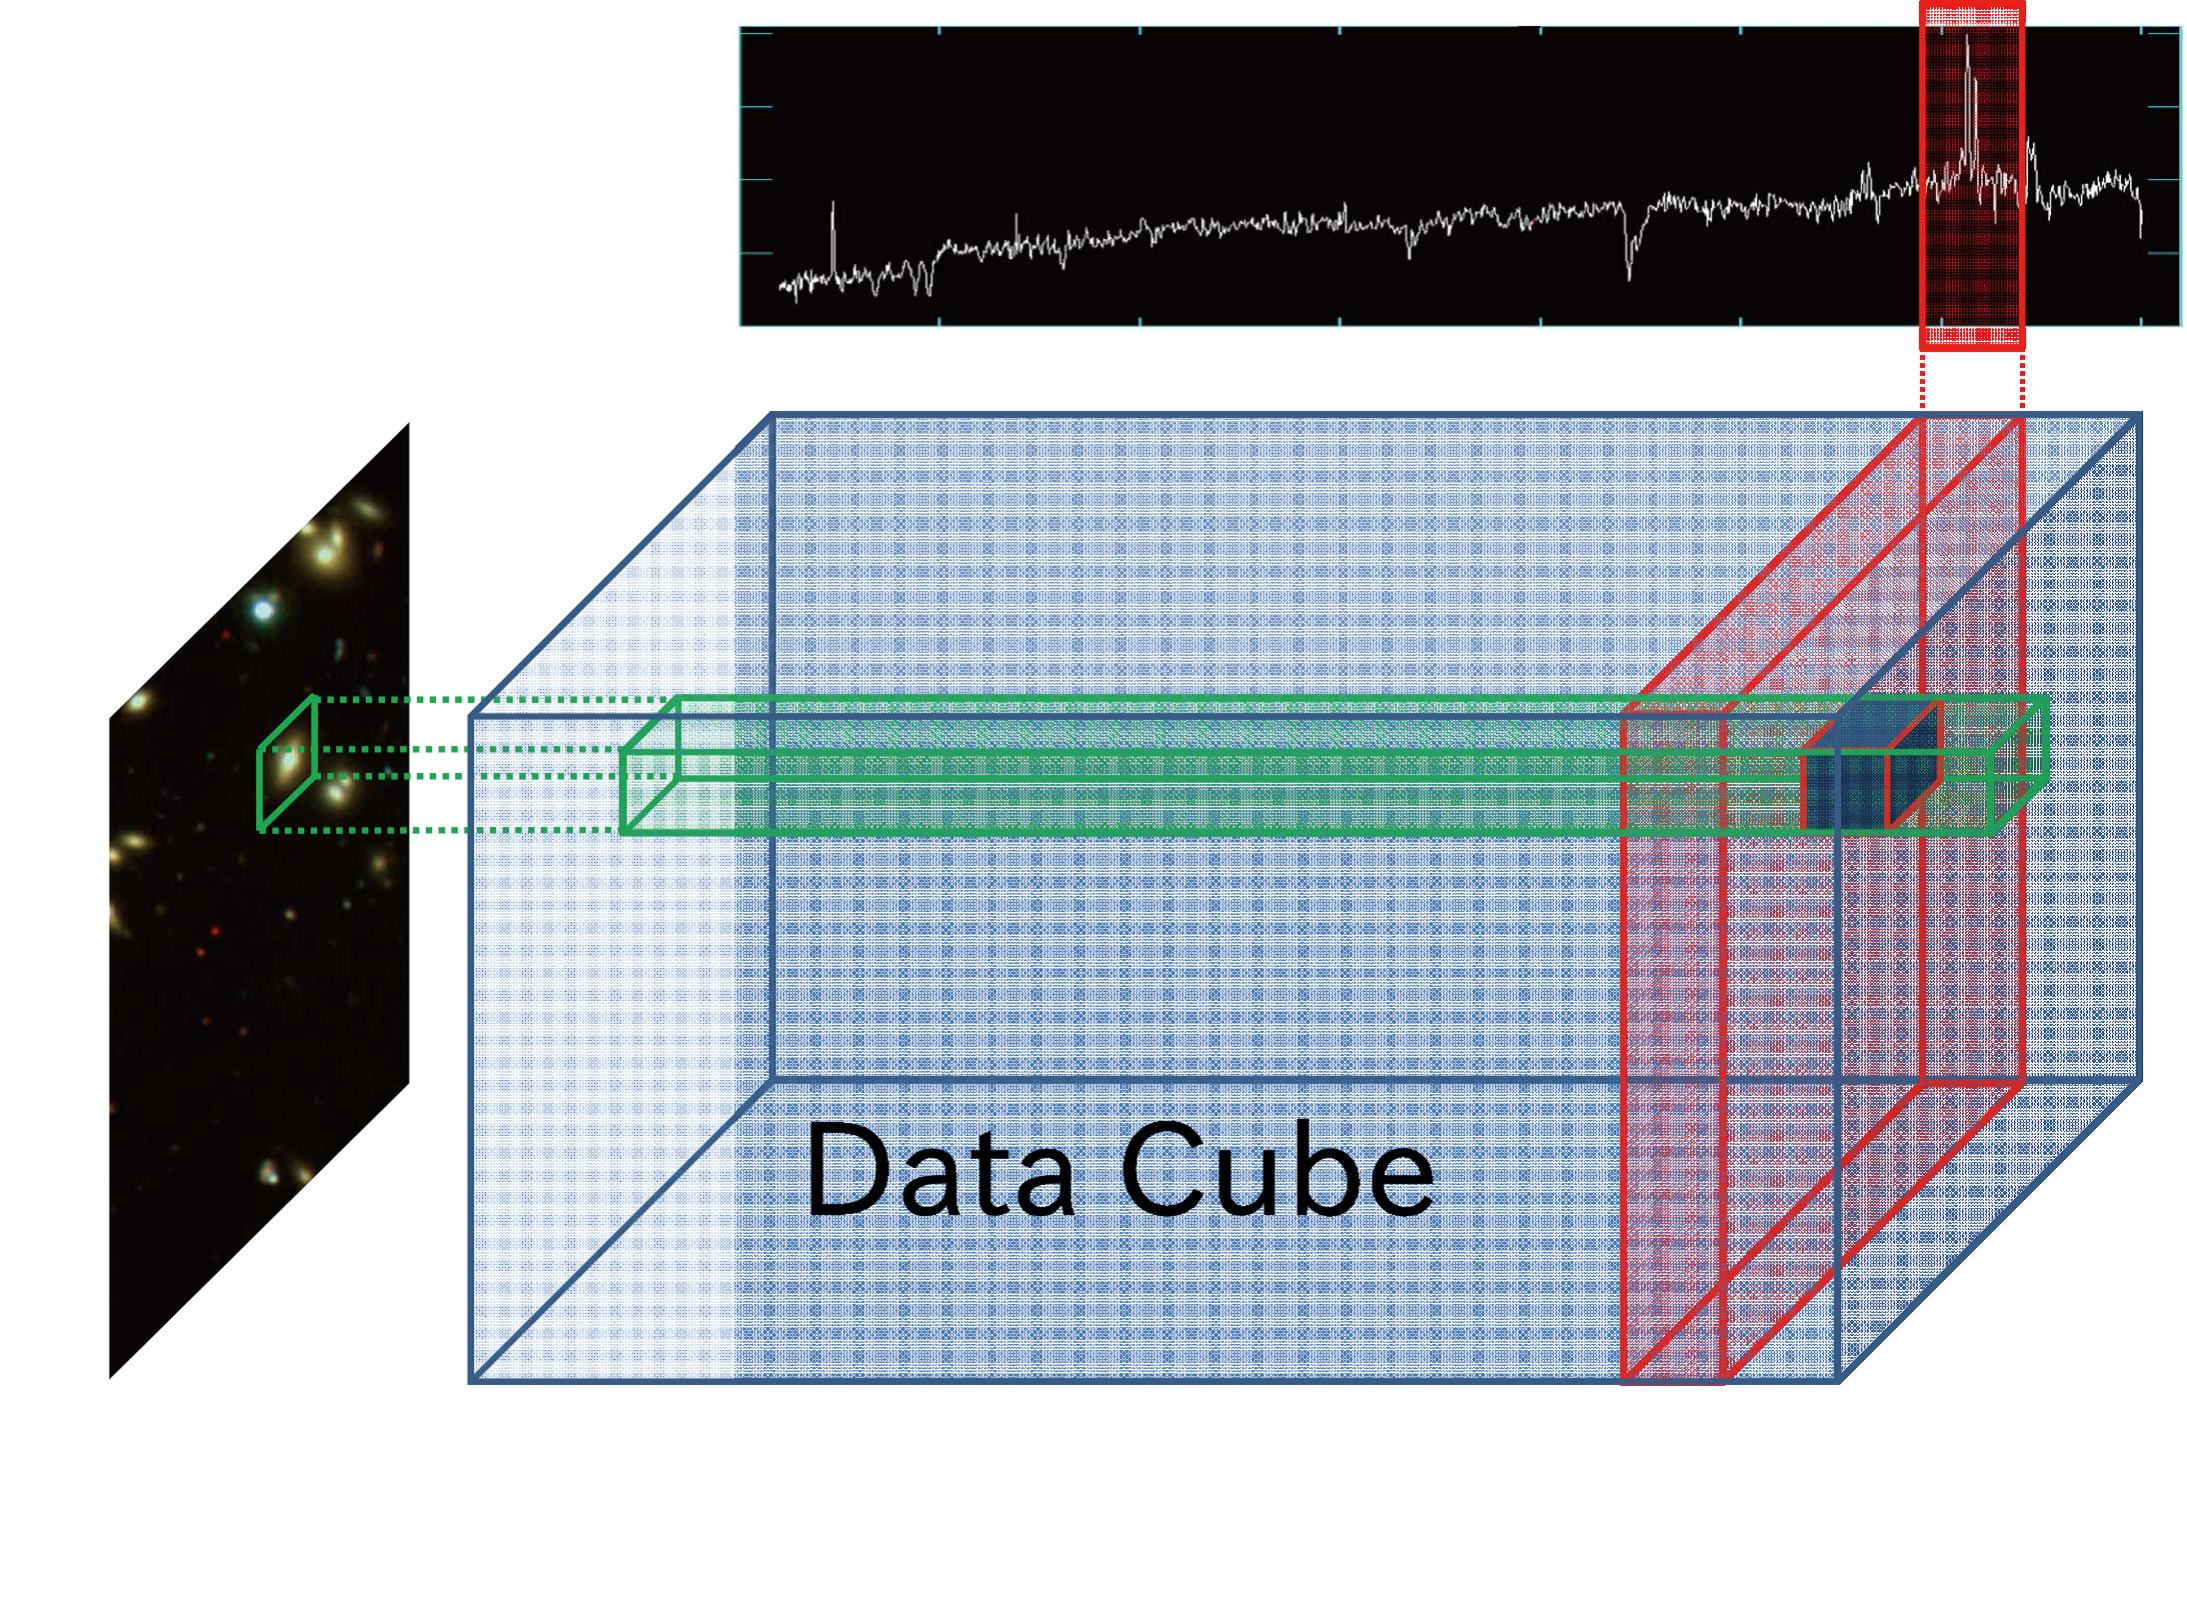
\includegraphics[width=0.5\textwidth]{images/cube.png}
   \end{tabular}
   \end{center}
   \caption[example]
   { \label{fig:cube} ALMA Data cube structure \cite{dent20132}.}
\end{figure}


Regarding the data format in astronomy, all are governed by a similar structure
consisting of metadata (information that describes the data) plus binary data.
ALMA has two special data models:
\begin{description}
    \item[ALMA Science Data Model:] \hfill \\
        XML format designed to save those metadata obtained from the observation
        process, and generate a link into binary data.
    \item[Measurement Set:] \hfill \\
        Binary table-based format (the main one and several secondary tables),
        which also saves metadata and binary data. This format will conduct
        reduction and processing in the Common Astronomy Software Applications
        (CASA), software created by NRAO\footnote{\url{http://casa.nrao.edu/}} for this purpose.
\end{description}

\subsection{Chilean Virtual Observatory}
\label{sec:chivo}
Although Chile is one of the most dynamic countries in its astronomic activity
in the world, until a year ago it did not have a VO.  For the moment, nor has
ALMA services to support the protocols and standards of other VO; therefore, it
is a challenge to pose the needs and requirements of this type of system.

Though the international community has been working and refining virtual
observatories and their standards, every new telescope and instrument imposes
new challenges and opportunities of development.  This is the ALMA data case,
which introduces the \emph{Big Data} problem as a current problem.  This means to
equip the virtual observatory that is hosting its data, with last generation
technology and frontier research in its tools.

The aim of this paper is to introduce the reader to the general architecture of
Virtual Observatories and, particularly to the current development of the
Chilean Virtual Observatory (ChiVO), from the software development perspective.
Furthermore, it will present its status and how were the restrictions and
intricacies of the ALMA data addressed.

\section{CHIVO ARCHITECTURE} 
The ChiVO is a virtual observatory under construction that will host the data of the observatories located in Chile, adhered to the interoperability standards of the International Virtual Observatories Alliance (IVOA), and using last generation technologies. 

This section describes the process of design conducted for this initiative.
The IVOA mission is to simplify the necessary coordination and collaboration to enable global and integrated access to the data collected by the international astronomical observatories. This organization was created in June 2002, and at the present has twenty-one active members.  Its working method is based on Working Groups, in charge of establishing protocols and standards that describe the general architecture of a VO (See Figure~\ref{fig:ivoavacio}).  Broadly, the architecture has three layers:
\begin{itemize}
    \item Users:  astronomers and scientists in general, interested in 
        the data published by the observatories.
    \item Resources: observatories and centres producing astronomical 
        data (real or simulated).
    \item Intermediate layer:  this layer defines what a virtual observatory 
        is; that is, how users and resources communicate using protocols and 
        standards to search and accees data.
\end{itemize}

\begin{figure}
   \begin{center}
   \begin{tabular}{c}
   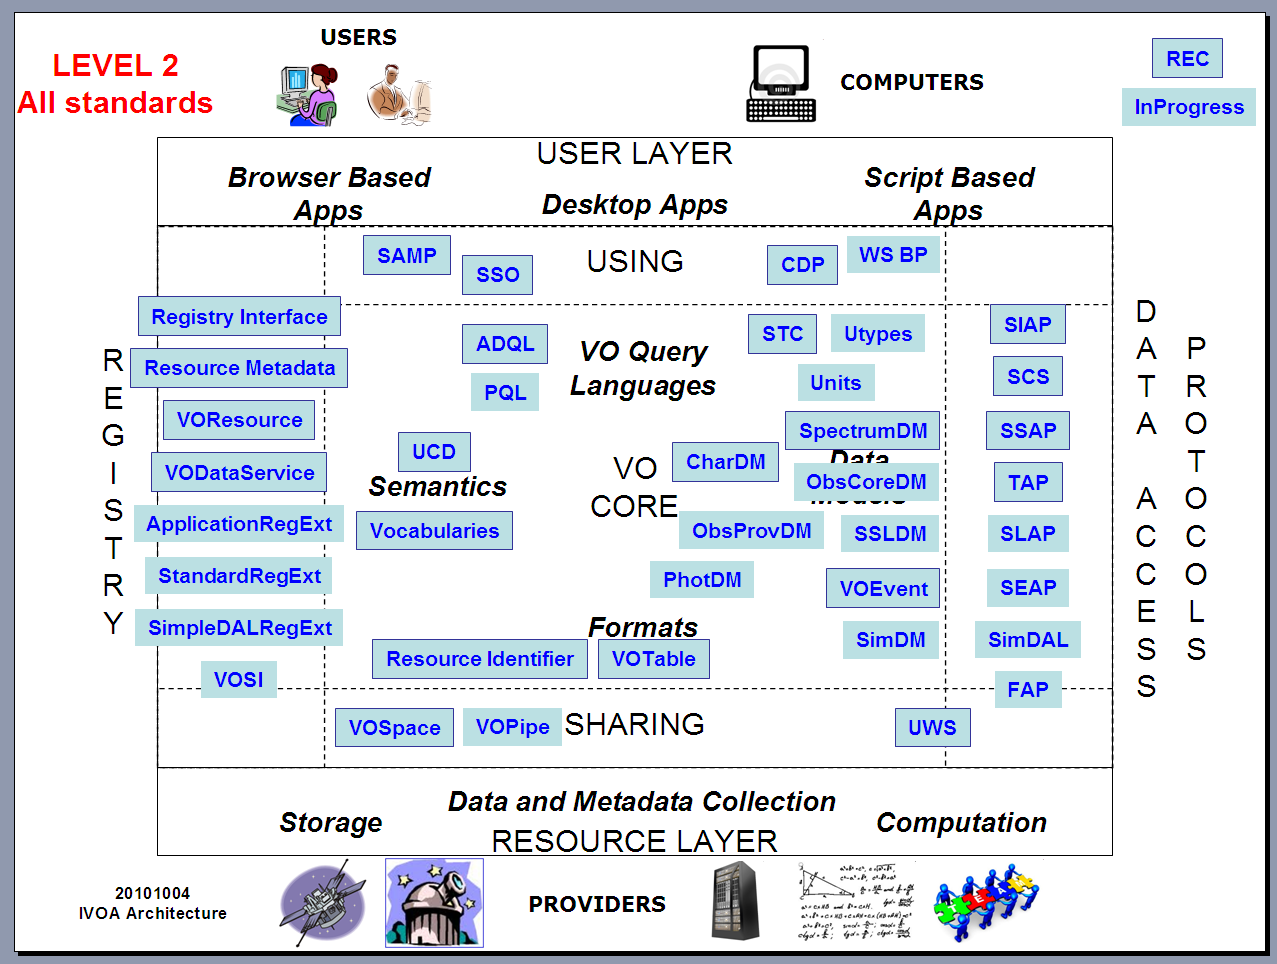
\includegraphics[width=0.5\textwidth]{images/ivoavacio.png}
   \end{tabular}
   \end{center}
   \caption[example]
   {\label{fig:ivoavacio} IVOA Architecture}
\end{figure}

\subsection{Requirements}
The creation of the ChiVO required the identification of the current needs of the national astronomy community, which can be summarized in:
\begin{description}
    \item[Discover:] \hfill \\
        Find astronomical data of an object or instrument on a high dimension specific region of the space, based on parameters of the spatial, temporary, spectral shafts, red shift, polarization, etc., either by search or exploration.
    \item[Obtain:] \hfill \\
        A download link of the required data in different formats, either in the VO or in an external service.
    \item[Compare:] \hfill \\
        Information crossing of the data obtained between the different sources of information.
\end{description}

A multidisciplinary team participated in this process (astronomers, engineers, scientists, experts in ALMA data, etc.); its duration was approximately 4 months, while the astronomy community was defining its requirements, and the use cases, and IT team contrasted it with international standards.

\subsection{ChiVO Architecture}
Depending on the needs of the Chilean radio astronomers, the requirements, use cases, and data models (compatible with the IVOA standards) induce the creation of the following architecture and development model (See Figure~\ref{fig:chivoarch}).

\begin{figure}
   \begin{center}
   \begin{tabular}{c}
   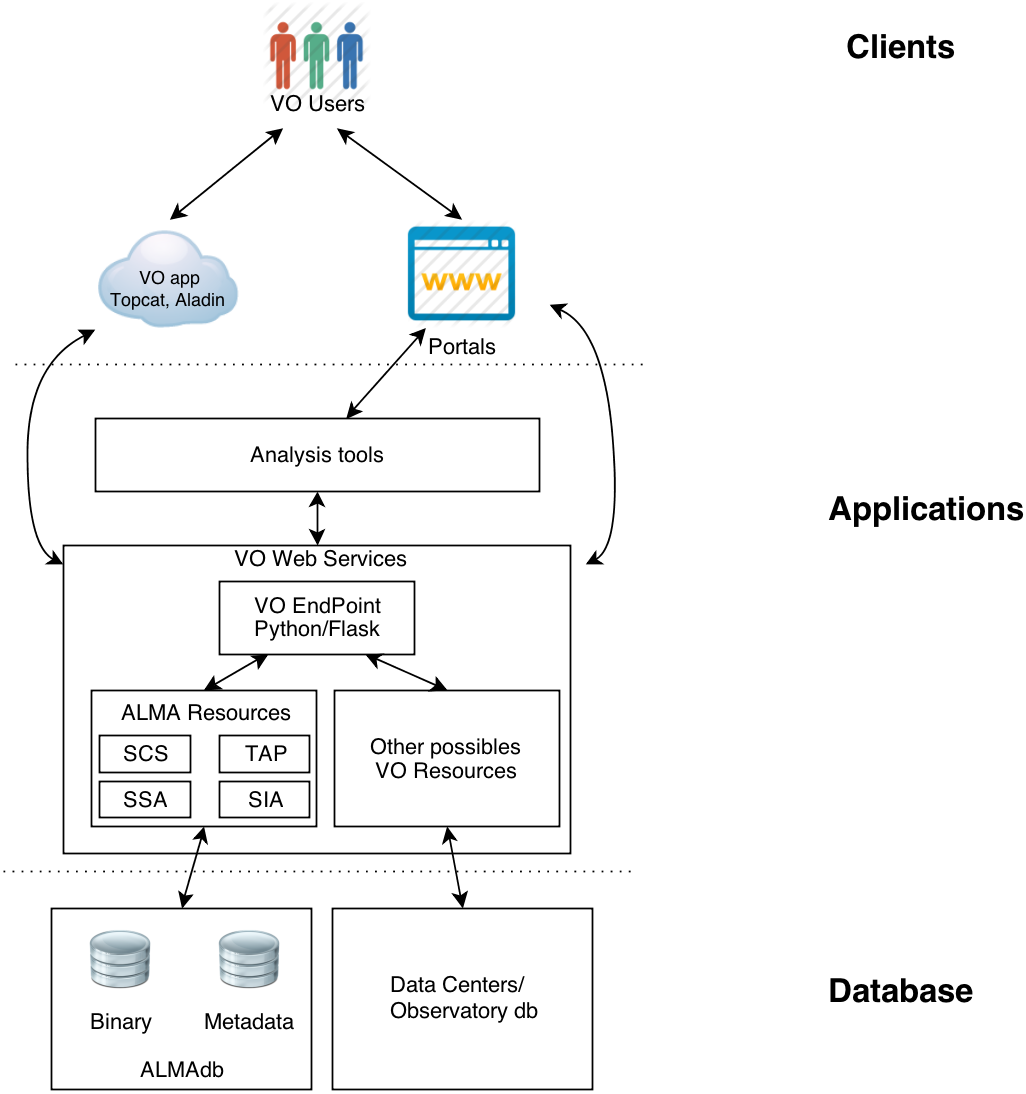
\includegraphics[width=0.5\textwidth]{images/chivo_capas.png}
   \end{tabular}
   \end{center}
   \caption[example]
   { \label{fig:chivoarch} ChiVO Architecture}
\end{figure}

\textbf{Abstraction layers:  Clients}
This layer represents the final user, and how communication between the user and data can be simplified.  In this layer the user conducts consultations through the access protocols offered by the ChiVO, or through an advanced form, using compatible applications with VO and its web portal.  Once the consultation is performed, the system shall return to the user a list describing the objects or observations found (metadata), and will be able to accessing them through a downloading link associated to each result.  It is relevant to say that the separation by layers of abstraction is achieved through flexibility and scalability in the system; thus, despite the layer, new applications may interact with ChiVO, as well as the addition of new information sources, aside from ALMA.

Consultations are received by the ChiVO through its data \emph{endpoint}, which receives requests in \texttt{HTTP}, \texttt{GET}, or \texttt{POST}; the endpoint will return the list of results in a XML VOTable format table \cite{ochsenbein2011ivoa}.  In the portal web case, VOTable is displayed and shown to the user through a web tool that enables a simple and efficient handling of VOTables, called VOView.

\textbf{Abstraction Layer:  Applications}
In this layer, we find the programs that process the inquiries between users and data.  Each IVOA standard requires a minimum of its own implementation to be compatible with VO.  In access protocols, it is only necessary the reception of basic HTTP requests, with the search parameters required.

The key element of the analysis tools is essential for the ChiVO efficiency.  This, because the data that will be analyzed by astronomers are usually large, and its transfer is expensive.  This problem can be solved bringing the analysis and processing tools closer to the place where the data to be processed is stored.

Whereas in future it will be necessary to offer searches based on other data, not only originating from ALMA, some abstraction is necessary when implementing this layer.  This, because it should enable the interaction of new information sources, as long as compatibility of IVOA is sustained.

In this layer is also in the proces of development a system able to resolve names (Sesame \footnote{\url{http://cds.u-strasbg.fr/cgi-bin/Sesame}} type, but for ALMA data), and the ChiVO registry.


\textbf{Abstraction Layer: Data}
In this layer are the resources that the data and metadata have.  The work is associated with a relational database to store metadata linked to the data model recommended by \emph{IVOA Observation Core Data Model} \cite{louys2011ivoa}, using a framework developed by the German VO DaCHS \footnote{\url{http://vo.ari.uni-heidelberg.de/soft/}}.  Concerning the performance, we are in the section that consumes more resources in both, computational time (resolves the database enquiries), and physical data storage.  

As momentary verification, the current implementation works with a set of data, with 1 TeraByte capacity, which comes from the reduction of the cycle 0 of ALMA.  Because of this limitation, the operation scheme of figure~\ref{fig:dachs} is the alternative proposed, where there might be N servers with DaCHS pointing to an M data base distributed or replicated.

\begin{figure}
   \begin{center}
   \begin{tabular}{c}
   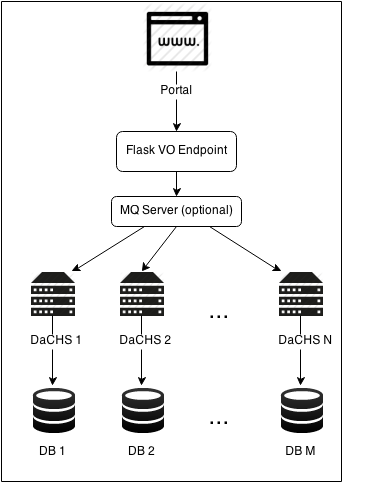
\includegraphics[width=0.5\textwidth]{images/interaccion.png}
   \end{tabular}
   \end{center}
   \caption[example]
   { \label{fig:dachs} Configuration of different machines with replicated or distributed data base}
\end{figure}

\subsection{ALMA data Metadata}
Building the relational data base with the ObsCore data model required field mapping from the ALMA Science Data Model (ASDM) \cite{viallefond2009sdm}.  An ASDM has a series of tables (XML) with the observation metadata. Here we used: \emph{main}, \emph{Source}, \emph{ExecBlock}, \emph{spectralWindow}.

\begin{table}[h]
\caption{Fields of the ObsCore, and origin from ASDM} 
\label{tab:obsasdm}
\begin{center}       
\begin{tabular}{lr}
        \textbf{Field ObsCore} & \textbf{ASDM} \\
        dataproduct\_type      & visibility \\
        calib\_level           & 1 \\
        obs\_collection        & ALMA \\
        obs\_id                & [ExecBlock.execBlockUID] \\
        obs\_publisher\_did    & [Cycle ID] \\
        access\_url            & [ChiVO URL] \\
        access\_format         & application/x-asdm \\
        access\_estsize        & [main.dataSize] \\
        target\_name           & [Source.sourceName] \\
        s\_ra                  & [Source.direction] \\
        s\_dec                 & [Source.direction] \\
        s\_fov                 & [1.2 * lambda / Antenna Diameter] \\
        s\_region              & circle \\
        s\_resolution          & [1.2*lambda/(ExecBlock.baseRangeMax)] \\
        t\_min                 & [ExecBlock.startTime] \\
        t\_max                 & [ExecBlock.endTime] \\
        t\_exptime             & [main.interval] \\
        t\_resolution          & [mainTable.interval] \\
        em\_min                & [ExecBlock.baseRangeMin] \\
        em\_max                & [ExecBlock.baseRangeMax] \\
        em\_res\_power         & [spectralWindow.resolution] \\
        o\_ucd                 & em.mm \\
        pol\_states            & [Source.stokesParameter[numStokes]] \\
        facility\_name         & ALMA \\
        instrument\_name       & ALMA \\
\end{tabular}
\end{center}
\end{table}

Table~\ref{tab:obsasdm} shows the result of the investigation; to the left are displayed the columns of the Observation class; the second column indicates where are the data taken from to assign the fields of the first column for the ASDM case.

Filling the fields of the Observation class requires to write a routine able to operate on the ASDM (XML) tables. Currently, there are multiple tools in the Common Applications Software Package of Astronomy (CASA) \cite{petry2012analysing}.

\subsection{Technologies used}
In the development of the ChiVO, there were various possible tools evaluated, which concluded in the following for each layer:

\textbf{Abstraction Layer:  Application}
The frameworks evaluated to implement the endpoint were: 
\begin{description}
    \item[{\ror}:] \hfill \\
        A framework of web development widely deployed nowadays, based on the concept Model-View-Controller (MVC).  However, this tool will not be used, because many functionalities are unnecessary for the present prototype.
    \item[Python/Flask:] \hfill \\
        The flask is a microframework specially designed for small web tools and services.  The current solution provides a framework for creating web applications; these can be accessed through various HTTP approaches.  Extensive documentation exists, as well as an active community to implement and solve the problems quickly.
\end{description}

\textbf{Abstraction Layer: Data}
Some of the \emph{toolkits} of Data Access Layer recommended by IVOA to accessing data through protocols are:  Simple Cone Search (SCS) \cite{williams2008simple}; Simple Image Access (SIA) \cite{tody2004simple}; Simple Spectral Access (SSA) \cite{tody2008simple}; and Table Access Protocol (TAP) \cite{dowler2010table} through the Astronomical Data Query Language (ADQL) \cite{yasuda2004astronomical}, and Universal Worker Service \cite{rixon2008universal}, the following was tested and validated:

\begin{description}
    \item[SAADA:] \hfill \\
        Developed by the French VO, this is a most useful tool from the viewpoint of the system user.  It has excellent documentation and a convenient installation process. It is developed in Java, and its deployment is conducted through Tomcat.  It is possible to configure SCS/SIA/SSA/TAP services, and is not an OpenSource project.
    \item[VO-Dance:] \hfill \\
        Developed by the Italian VO, this is a tool in Java in its Backend, and Phyton in its Frontend (Framework Django). What is remarkable of this tool is that it works using MySQL as a core data base engine; according to the latest news related to its development, it might exist eventually, a support for PostgresSQL.  This is not an OpenSource tool, and its documentation is uncertain, since it is still in development.  Is compatible with SCS/SIA/SSA/TAP services.
    \item[openCADC:] \hfill \\
        Developed by the Canadian VO, this is an Open Source tool written in Java, currently used in the ALMA Science Archive.  This toolkit is one of the most robust, and has different packages with services for its use in the webservice; however, it has a poor documentation, which is compensated with an open community of development.  It is possible to configure TAP, UWS services.
    \item[DaCHS:] \hfill \\
        Developed by the German VO, this is an OpenSource tool written in Python.  It is one of the DAL toolkits most used by VO, since it has an extensive installation and configuration documentation. It is possible to configure SCS/SIA/SSA/TAP services.
\end{description}

\begin{table}[h]
\caption{Summary of the toolkits in a comparison chart} 
\label{table:toolkits}
\begin{center}       
\begin{tabular}{lrrrrr}
    {\bf Toolkits} & {\bf Language} & {\bf OpenSource} & {\bf Documentation} & {\bf Services} & {\bf Latest update}  \\
    SAADA          & Java           & No               & Yes                  & SCS/SIA/SSA/TAP & May 2012     \\
    VO-Dance       & Java/Python    & No               & No                  & SCS/SIA/SSA/TAP & December 2012 \\
    openCADC       & Java           & Yes               & No                  & TAP             & ---           \\
    DaCHS          & Python         & Yes               & Yes                  & SCS/SIA/SSA/TAP & June 2013    \\
\end{tabular}
\end{center}
\end{table}

\textbf{Abstraction Layer:  Clients}
Initially, the user interface or frontend should have only views, therefore, its development might be virtually in any language or framework; for example: PHP, Django, or Ruby on Rails.  However, with the platform requirements, specially the users' layer, the selected framework was the MVC, agile enough and compatible with the rest of the services, Ruby on Rails.


\section{PROGRESS STATUS}
It was necessary to identify not only the requirements and use cases, but the interactions that users will have with the system, to begin the ChiVO development.  We can observe the interaction diagram sequence between the user and the ChiVO in figure~\ref{fig:secuencia}.  According to this diagram, the requirements and technologies used will be specified in the progress status for each abstraction layer.

\begin{figure}
   \begin{center}
   \begin{tabular}{c}
   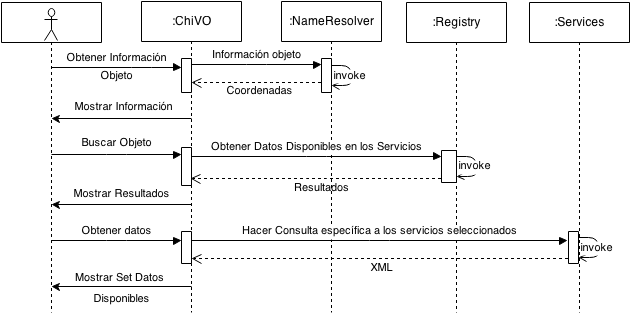
\includegraphics[width=0.7\textwidth]{images/secuencia.png}
   \end{tabular}
   \end{center}
   \caption[example]
   { \label{fig:secuencia} Sequence diagram between User and ChiVO}
\end{figure}

The ChiVO software architecture is based on the use of the IVO protocols and standards.  These protocols and standards are grouped in layers, with emphasis on the application and data layers (See Figure~\ref{fig:ivoarch}); this, because their basic standards define the minimum operation that a VO should conduct.  Following is a detail of the elements that ChiVO has implemented in these layers.

\begin{figure}
   \begin{center}
   \begin{tabular}{c}
   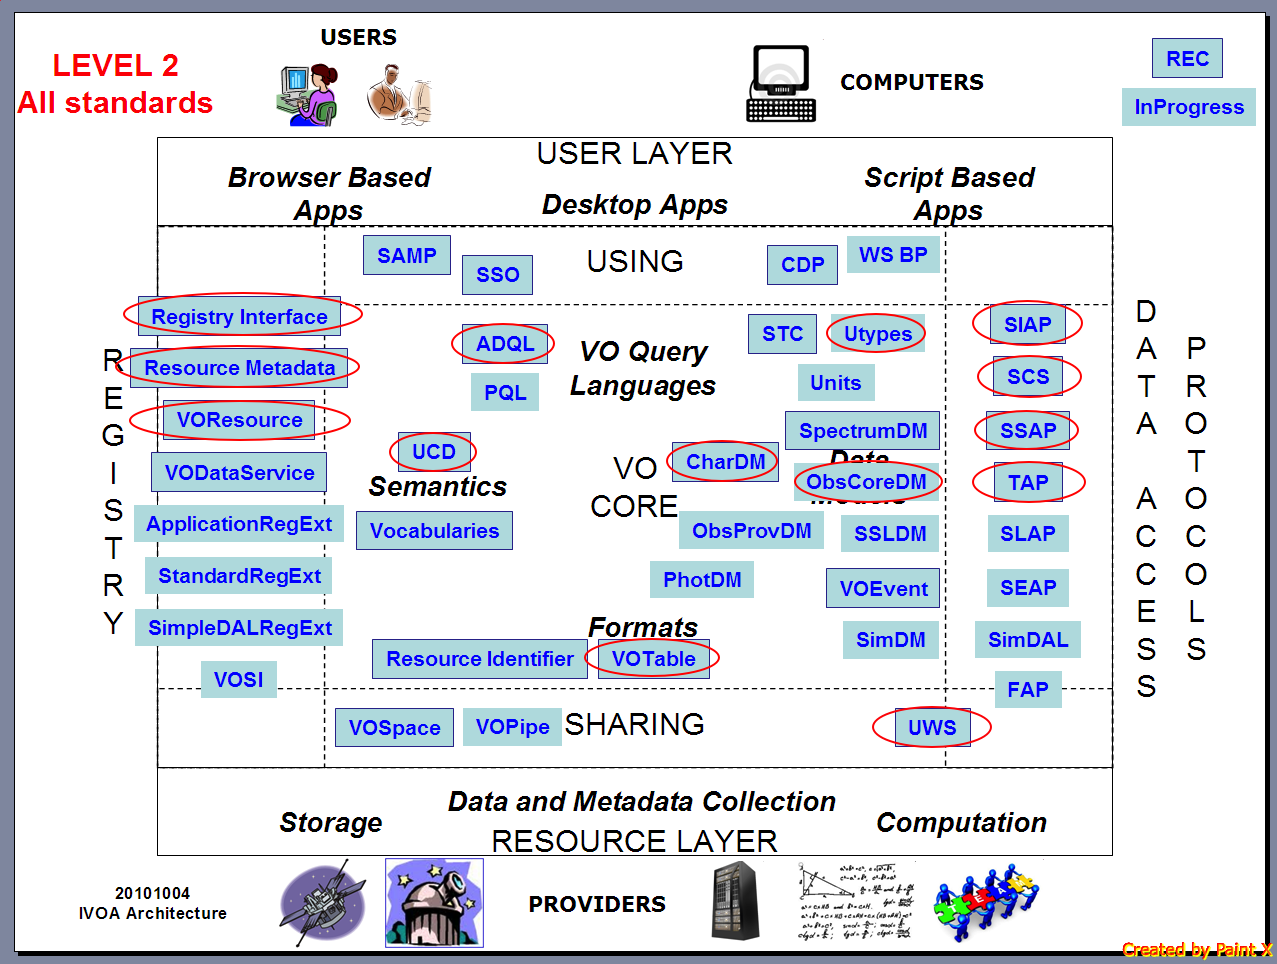
\includegraphics[width=0.5\textwidth]{images/arquitectura_2.png}
   \end{tabular}
   \end{center}
   \caption[example]
   {\label{fig:ivoarch} IVOA architecture with Protocols and Standards used}
\end{figure}

\begin{description}
    \item[Application Layer:] \hfill \\
        A Web Service compatible with the VO needs at least a \emph{Table Access Protocol} to accessing ChiVO data model, using the \emph{Astronomical Data Query Language}.  Furthermore, to achieve compliance with the system requirements, the protocol currently implemented for conical searches is \emph{Simple Cone Search}; the access protocol to spectral data is \emph{Simple Spectral Access}, and the images access protocol is \emph{Simple Image Access}. 
    \item[Data Layer:] \hfill \\
        This layer requires the configuration of the relational database with a data model recommended by IVOA, called \emph{Observation Core Data Model}.  This data model enables the VO interoperability, since it defines a minimum amount of attributes in the tables, with a specific name and type of data; thus, is possible the access to the various standardized services through a \emph{TAP + Obscore}.  In addition, the information transfer format (metadata) is with the standard \emph{XML VOTable format}.
\end{description}

\subsection{Abstraction Layer:  Clients}
Within the sequence diagram, the Frontend is the VO-Client; that is, it is in charge of generating the interaction between users and other elements within the system.
At the present, the frontend generated in ROR enables the interaction with:
\begin{description}
    \item[Resolving names]:\hfill \\
        from a name (String) returns the position of an object in celestial coordinates, using the SESAME service of Astrogrid.
    \item[Registry]: \hfill \\
        searches services within the endpoint, and then, according to the user's needs, it chooses on which to work for consultations.
    \item[Services]: \hfill \\
        consults with the different web services that provide data through a certain protocol, and standardizes the results in a XML VOTable for its organized deployment, using a VOView javascript library.
\end{description}

\subsection{Abstraction Layer:  Applications}
The Endpoint is responsible for the generation of a transparent interaction between the VO clients, and the possible resources that might be configured.  Here, the Endpoint generates an interface for services configured by the Backend, and for those available, through the VO-Paris record.  VO-Paris has a Web API in REST to consult for resources, returning a JSON file with outcomes.

\subsection{Abstraction Layer:  Data}
Currently, ALMA furnishes to the ChiVO public data, which include ASDM, Measurement \cite{petry2012analysing}, FITS \cite{wells1981fits}, however, it is necessary to draw out the ObsCoreDM metadata to make possible their entry to the data base (See Figure~\ref{fig:metadata}).

The procedure is carried out through a program, and using the DaCHS backend framework, which enables the configuration of resources and services through Resource Descriptor  configuration files.  Once created the entries in the data base, and configured the SCS, SSAP, SIAP, TAP services, it can be accessed through queries defined in each protocol.

\begin{figure}
   \begin{center}
   \begin{tabular}{c}
   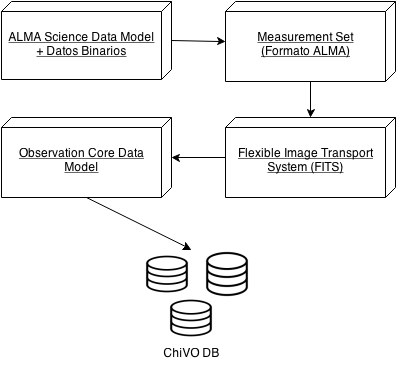
\includegraphics[width=0.5\textwidth]{images/metadata.png}
   \end{tabular}
   \end{center}
   \caption[example]
   {\label{fig:metadata} Transformation process from the ALMA Frontend to the ChiVO database}
\end{figure}

\section{CONCLUSION AND FUTURE WORK}
Despite the amount of data generated by observatories in Chile, there was no VO a year ago, and particularly, ALMA at the moment does not have services compatible with VO. The implementation of the ChiVO caused a series of complications that arise from the understanding of the needs of the astronomers, and how these are translated to data systems and services, using IVOA international regulations.

The approach of the current development is focused on incremental prototypes, thus generating frequent deliverables to the system users (Astronomers) who are pleased by the progress made. However, there are always things to implement, or new ideas coming up. So far it has been possible to capture the astronomers requirements, and to address the study of the protocols and standards, thus creating the data access services (SCS, SIA, SSA, TAP); these have access to the data base that use a relational data model (ObsCore), subjected to their own ChiVO architecture, which enables the interoperability of the services.

Currently, the prototype is in its first delivery, and by mid-2014 it will be launched its second iteration, which will include the public data of the cycle 0 of ALMA. Hence, more users will be familiarized with the system, having the chance to test in situ the current functionalities and limitations of the implementations.  For the following versions it is considered the implementation of other IVOA architecture protocols, as the section of Registry and standards of access to resources, as VOSPace \cite{graham2007vospace}.  Regarding the models and multidimensional data, as the ALMA cubes, it will be necessary to work in the creation or adaptation of the IVOA standards.

\acknowledgments     %>>>> equivalent to \section*{ACKNOWLEDGMENTS}       
This work is partially financed by the FONDEF D11I1060 project.
\newpage
\bibliography{report}   %>>>> bibliography data in report.bib
\bibliographystyle{spiebib}   %>>>> makes bibtex use spiebib.bst

\end{document} 
